
\documentclass[11pt]{article}

\usepackage{fullpage,graphicx,latexsym,picinpar,amsbsy,amsmath,amsfonts}

           

%%%%%%%%%%%%%%%%%%%%%%%%%%%%%%%%%%%%%%%%%%%%%%%%%%%%%%%%%%%%%%%%%%%%%%%%%%%%%%%%%%%
%%%%%%%%%%%  LETTERS 
%%%%%%%%%%%%%%%%%%%%%%%%%%%%%%%%%%%%%%%%%%%%%%%%%%%%%%%%%%%%%%%%%%%%%%%%%%%%%%%%%%%

\newcommand{\barx}{{\bar x}}
\newcommand{\bary}{{\bar y}}
\newcommand{\barz}{{\bar z}}
\newcommand{\bart}{{\bar t}}

\newcommand{\bfP}{{\bf{P}}}

%%%%%%%%%%%%%%%%%%%%%%%%%%%%%%%%%%%%%%%%%%%%%%%%%%%%%%%%%%%%%%%%%%%%%%%%%%%%%%%%%%%
%%%%%%%%%%%%%%%%%%%%%%%%%%%%%%%%%%%%%%%%%%%%%%%%%%%%%%%%%%%%%%%%%%%%%%%%%%%%%%%%%%%
                                                                                
\newcommand{\parend}[1]{{\left( #1  \right) }}
\newcommand{\spparend}[1]{{\left(\, #1  \,\right) }}
\newcommand{\angled}[1]{{\left\langle #1  \right\rangle }}
\newcommand{\brackd}[1]{{\left[ #1  \right] }}
\newcommand{\spbrackd}[1]{{\left[\, #1  \,\right] }}
\newcommand{\braced}[1]{{\left\{ #1  \right\} }}
\newcommand{\leftbraced}[1]{{\left\{ #1  \right. }}
\newcommand{\floor}[1]{{\left\lfloor #1\right\rfloor}}
\newcommand{\ceiling}[1]{{\left\lceil #1\right\rceil}}
\newcommand{\barred}[1]{{\left|#1\right|}}
\newcommand{\doublebarred}[1]{{\left|\left|#1\right|\right|}}
\newcommand{\spaced}[1]{{\, #1\, }}
\newcommand{\suchthat}{{\spaced{|}}}
\newcommand{\numof}{{\sharp}}
\newcommand{\assign}{{\,\leftarrow\,}}
\newcommand{\myaccept}{{\mbox{\tiny accept}}}
\newcommand{\myreject}{{\mbox{\tiny reject}}}
\newcommand{\blanksymbol}{{\sqcup}}
                                                                                                                         
\newcommand{\veps}{{\varepsilon}}
\newcommand{\Sigmastar}{{\Sigma^\ast}}
                           
\newcommand{\half}{\mbox{$\frac{1}{2}$}}    
\newcommand{\threehalfs}{\mbox{$\frac{3}{2}$}}   
\newcommand{\domino}[2]{\left[\frac{#1}{#2}\right]}  

%%%%%%%%%%%% complexity classes

\newcommand{\PP}{\mathbb{P}}
\newcommand{\NP}{\mathbb{NP}}
\newcommand{\PSPACE}{\mathbb{PSPACE}}
\newcommand{\coNP}{\textrm{co}\mathbb{NP}}
\newcommand{\DLOG}{\mathbb{L}}
\newcommand{\NLOG}{\mathbb{NL}}
\newcommand{\NL}{\mathbb{NL}}

%%%%%%%%%%% decision problems

\newcommand{\PCP}{\sc{PCP}}
\newcommand{\Path}{\sc{Path}}
\newcommand{\GenGeo}{\sc{Generalized Geography}}

\newcommand{\malytm}{{\mbox{\tiny TM}}}
\newcommand{\malycfg}{{\mbox{\tiny CFG}}}
\newcommand{\Atm}{\mbox{\rm A}_\malytm}
\newcommand{\complAtm}{{\overline{\mbox{\rm A}}}_\malytm}
\newcommand{\AllCFG}{{\mbox{\sc All}}_\malycfg}
\newcommand{\complAllCFG}{{\overline{\mbox{\sc All}}}_\malycfg}
\newcommand{\complL}{{\bar L}}
\newcommand{\TQBF}{\mbox{\sc TQBF}}
\newcommand{\SAT}{\mbox{\sc SAT}}

%%%%%%%%%%%%%%%%%%%%%%%%%%%%%%%%%%%%%%%%%%%%%%%%%%%%%%%%%%%%%%%%%%%%%%%%%%%%%%%%%%%
%%%%%%%%%%%%%%% for homeworks
%%%%%%%%%%%%%%%%%%%%%%%%%%%%%%%%%%%%%%%%%%%%%%%%%%%%%%%%%%%%%%%%%%%%%%%%%%%%%%%%%%%

\newcommand{\student}[2]{%
{\noindent\Large{ \emph{#1} SID {#2} } \hfill} \vskip 0.1in}

\newcommand{\assignment}[1]{\medskip\centerline{\large\bf CS 111 ASSIGNMENT {#1}}}

\newcommand{\duedate}[1]{{\centerline{due {#1}\medskip}}}     

\newcounter{problemnumber}                                                                                 

\newenvironment{problem}{{\vskip 0.1in \noindent
              \bf Problem~\addtocounter{problemnumber}{1}\arabic{problemnumber}:}}{}

\newcounter{solutionnumber}

\newenvironment{solution}{{\vskip 0.1in \noindent
             \bf Solution~\addtocounter{solutionnumber}{1}\arabic{solutionnumber}:}}
				{\ \newline\smallskip\lineacross\smallskip}

\newcommand{\lineacross}{\noindent\mbox{}\hrulefill\mbox{}}

\newcommand{\decproblem}[3]{%
\medskip
\noindent
\begin{list}{\hfill}{\setlength{\labelsep}{0in}
                       \setlength{\topsep}{0in}
                       \setlength{\partopsep}{0in}
                       \setlength{\leftmargin}{0in}
                       \setlength{\listparindent}{0in}
                       \setlength{\labelwidth}{0.5in}
                       \setlength{\itemindent}{0in}
                       \setlength{\itemsep}{0in}
                     }
\item{{{\sc{#1}}:}}
                \begin{list}{\hfill}{\setlength{\labelsep}{0.1in}
                       \setlength{\topsep}{0in}
                       \setlength{\partopsep}{0in}
                       \setlength{\leftmargin}{0.5in}
                       \setlength{\labelwidth}{0.5in}
                       \setlength{\listparindent}{0in}
                       \setlength{\itemindent}{0in}
                       \setlength{\itemsep}{0in}
                       }
                \item{{\em Instance:\ }}{#2}
                \item{{\em Query:\ }}{#3}
                \end{list}
\end{list}
\medskip
}

%%%%%%%%%%%%%%%%%%%%%%%%%%%%%%%%%%%%%%%%%%%%%%%%%%%%%%%%%%%%%%%%%%%%%%%%%%%%%%%%%%%
%%%%%%%%%%%%% for quizzes
%%%%%%%%%%%%%%%%%%%%%%%%%%%%%%%%%%%%%%%%%%%%%%%%%%%%%%%%%%%%%%%%%%%%%%%%%%%%%%%%%%%

\newcommand{\quizheader}{ {\large NAME: \hskip 3in SID:\hfill}
                                \newline\lineacross \medskip }


%%%%%%%%%%%%%%%%%%%%%%%%%%%%%%%%%%%%%%%%%%%%%%%%%%%%%%%%%%%%%%%%%%%%%%%%%%%%%%%%%%%
%%%%%%%%%%%%% for final
%%%%%%%%%%%%%%%%%%%%%%%%%%%%%%%%%%%%%%%%%%%%%%%%%%%%%%%%%%%%%%%%%%%%%%%%%%%%%%%%%%%

\newcommand{\namespace}{\noindent{\Large NAME: \hfill SID:\hskip 1.5in\ }\\\medskip\noindent\mbox{}\hrulefill\mbox{}}



\begin{document}

% v -- YOUR NAME and SID in the braces
\student{Chris Wong}{860923521}
% v -- ASSIGNMENT NUMBER in the braces
\assignment{Homework 2}
% v-- DUE DATE in the braces
\duedate{4/26/2011}

\medskip

%%%%%%%%%%%%%%%%%%%%%%%%%%%%%%%%%%%%%%%%%%%%%%%%%%%%%%%%%%%%%%%%%%%%%%%%%%

\lineacross

%%%%%%%%%%%%%%%%%%%%%%%%%%%%

\begin{problem}
Let $\naturals_k = \braced{1,2,...,k}$ be the set of natural numbers between
$1$ and $k$, where $k$ is some natural number.
For a natural number $x$, by $F(x)$ we denote the set of its prime
factors.

\medskip
\noindent
(a) We define relation $\bowtie$ on $\naturals_k$ as follows:
$x \bowtie y$ if and only if $F(x) = F(y)$.
List all equivalence classes of $\bowtie$ for $\naturals_{30}$.

\medskip
\noindent
(b)
Now define relation $\unlhd$ on the equivalence classes of
$\bowtie$:
$[x]\unlhd [y]$ if and only if $F(x) \subseteq F(y)$.

Prove that $\unlhd$ is a partial order.
Also, draw the Hasse diagram of $\unlhd$ for $\naturals_{14}$. For example,
the reverse page shows the Hasse diagram of $\unlhd$ for $\naturals_{10}$.

\medskip
\end{problem}

%---------------------------

\begin{solution}
\\a) equivalence classes of $\bowtie$ for $\naturals_{30}$.
\\$[1]= \braced{1}$, $[2] = \braced{2,4,8,16}$, $[3] = \braced{3,9,27}$,
\\$[5] = \braced{5}$, $[6] = \braced{6}$, $[7] = \braced{7}$,
\\$[10] = \braced{10}$, $[11] = \braced{11}$, $[12] = \braced{12}$,
\\$[13] = \braced{13}$, $[14] = \braced{14}$, $[15] = \braced{15}$,
\\$[17] = \braced{17}$, $[18] = \braced{18}$, $[19] = \braced{19}$,
\\$[20] = \braced{20}$, $[21] = \braced{21}$, $[22] = \braced{22}$,
\\$[23] = \braced{23}$, $[24] = \braced{24}$, $[26] = \braced{26}$,
\\$[28] = \braced{28}$, $[29] = \braced{29}$, $[30] = \braced{30}$,
\\
\\b) $[x]R[y] \Leftrightarrow f(x) \leq f(y)$
\\$[1]R[2] \rightarrow {empty} \leq {2,4,8,16} \rightarrow true$
\\$[2]R[5] \rightarrow {2,4,8,16} \leq {5} \rightarrow false$
\\$[75]R[15], [15]R[75] \rightarrow {15,45,75} \rightarrow [15] = [75]$
\\$[30]R[90], [90]R[30] \rightarrow {30,60,90} \rightarrow [30] = 90$
\\Thus, it is anti-symmetric & is on the equivialence classes.
\\
\\$[x]R[x]$
\\$\rightarrow [1]R[1] \rightarrow {empty} \leq {empty} \rightarrow true$
\\$\rightarrow [2]R[2] \rightarrow {2,4,8,16} \leq {2,4,8,16} \rightarrow true$
\\$\rightarrow [x] \leq [x]$
\\Thus, it is reflexive
\\
\\$[x]R[y],[y]R[z],[x]R[z]$
\\$\rightarrow [1]R[2],[2]R[6],[1]R[6] \rightarrow [1] \leq [6] \rightarrow true$
\\$\rightarrow [1]R[5],[5]R[10],[1]R[10] \rightarrow [1] \leq [10] \rightarrow true$
\\$\rightarrow [3]R[6],[6]R[12],[3]R[12] \rightarrow [3] \leq [12] \rightarrow true$
\\Thus, it is transitive con't $\rightarrow$
\\
\\We can conclude that the relation is of partial order because it is anti-symmetric, reflexive, and transitive
\\\\\\\\$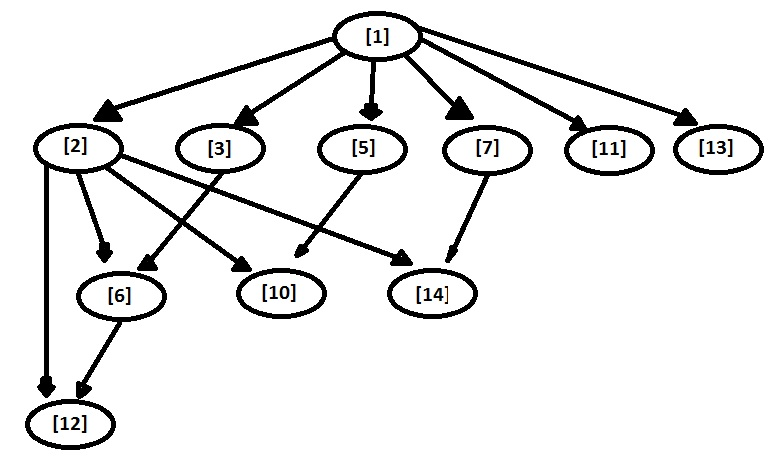
\includegraphics[scale = 0.7]{tmp3.jpg}$

\end{solution}

%%%%%%%%%%%%%%%%%%%%%%%%%%%%
\pagebreak

\begin{problem}
In the RSA, Bob chooses $p =11$, $q = 17$.
He is considering three choices for the public
exponent $e$: $5$, $7$ and $33$,
but he's not sure whether they are correct.

\begin{description}

\item{(a)} Which of these three choices for $e$ are correct?
Justify your answer.

\item{(b)} Let now $e$ be the smallest correct choice.
Determine the value of the secret exponent $d$.

\item{(c)} Suppose Alice wants to send $M = 26$ to
Bob. Determine the ciphertext $C$.

\item{(d)} What computation will Bob perform to
decrypt $C$? Show the result.

\end{description}

In parts (b), (c), (d), you don't need to show the details of the
computation (a calculator may be useful for this),
but you need to explain what steps are required to obtain the result.
\end{problem}


%-----------------------------

\begin{solution}
	\\a) n = pq = (11)(17) = 187
	\\ x = (p-1)(q-1) = (11-1)(17-1) =160
	\\e must statisfy the following conditions:
	\\1 $<$ e $<$ x, gcd(x,e) == 1, e == prime number
	\\
	\\for 5: gcd(160,5) = 5 != 1; fails condition
	\\for 33: 33 != prime number; fails condition
	\\for 7: 1 $<$ 7 $<$ 160 is true; gcd(160,7) == 1; 7 == prime number
	\\
	\\Since 7 statfies all the conditions and 5 $&$ 33 fail at least one we can
	\\conclude that 7 is the correct choice for 'e'
	\\e = 7
	\\
	\\b)smallest correct choice = 7
	\\p = 11, q = 17, e = 7
	\\thus n = 187 and x = 160
	\\d = $e^{-1}$(mod(x)) = $7^{-1}$(mod160)
    \\7z + 160y = 1 \rightarrow 7(23) + 160(1) \rightarrow z = d = 23
    \\
    \\c) $m^{e}(rem(n))$ \rightarrow 26^{7}(rem(187)) \rightarrow c = 104
    \\
    \\d) Ds(c) = c^{d}(rem(n)) \rightarrow 104^{23}(rem(187)) = 26
    \\
 \end{solution}

%%%%%%%%%%%%%%%%%%%%%%%%%%%
\pagebreak

\begin{problem}
 	Individual assignment, do not need to complete problem 3
\end{problem}

%----------------------------

\begin{solution}
	Individual assignment, do not need to complete problem 3
\end{solution}

\end{document}

